\documentclass[../main.tex]{subfiles}

\begin{document}
    \subsection{Elastisch}

    \begin{figure}[H]
        \begin{center}
            \centerline{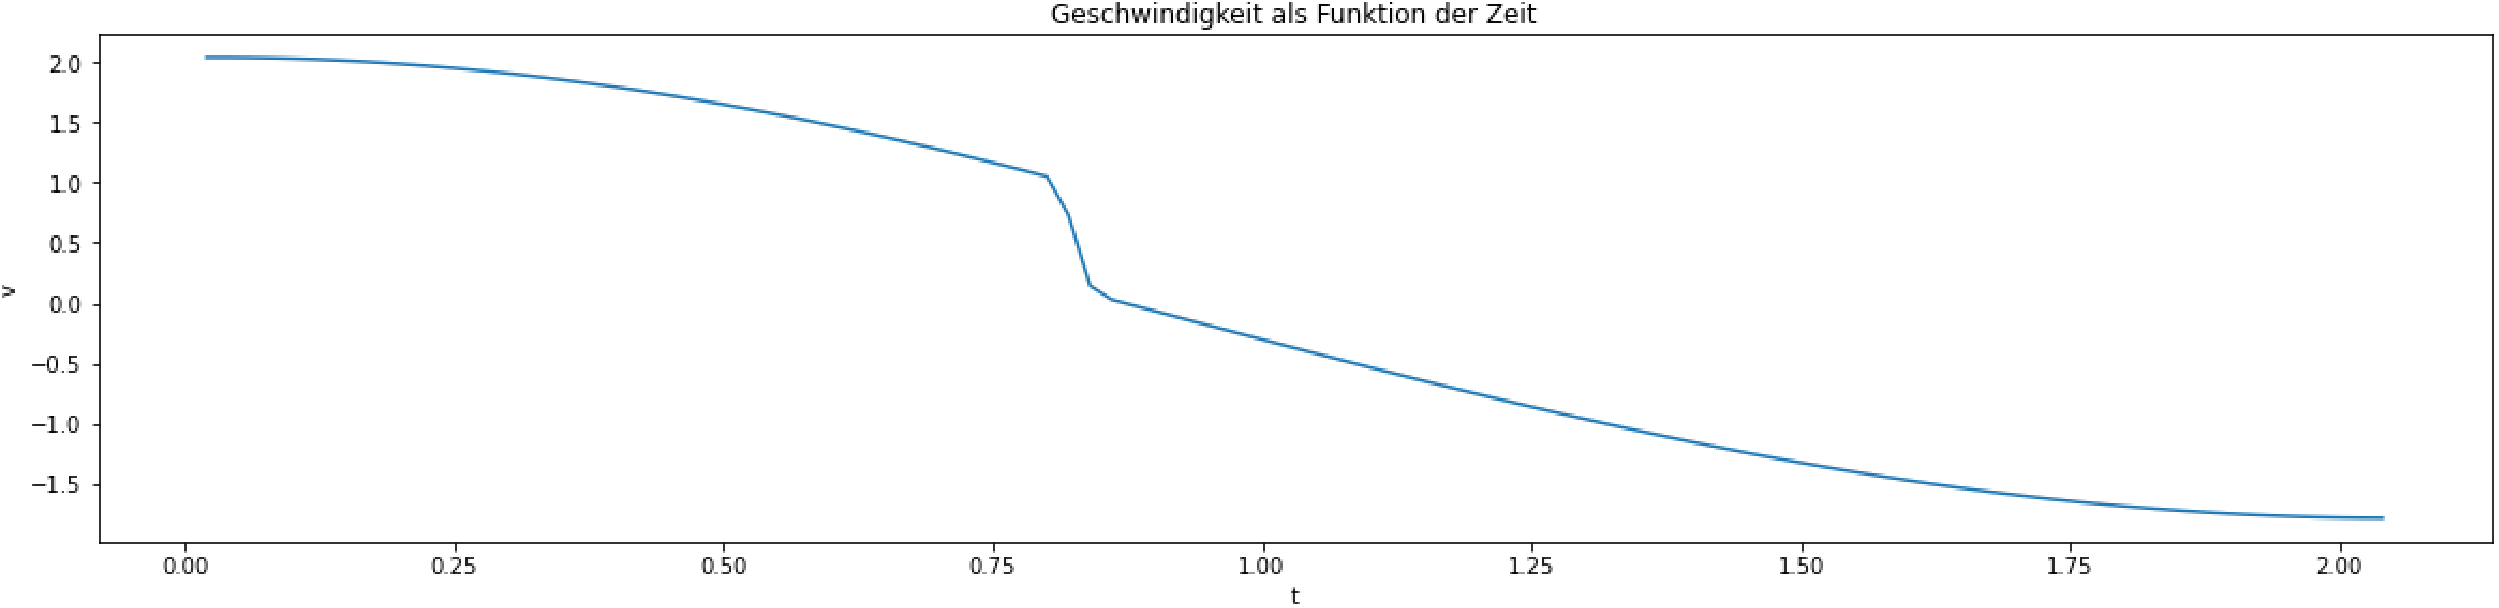
\includegraphics[width=155mm]{./images/Elastisch/GeschwindigkeitAlsFunktionDerZeit}}
            \caption{Geschwindigkeit als Funktion der Zeit}
            \label{fig:GeschwindigkeitAlsFunktionDerZeit}
        \end{center}
    \end{figure}

    \begin{figure}[H]
        \begin{center}
            \centerline{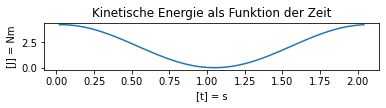
\includegraphics[width=155mm]{./images/Elastisch/KinetischeEnergieAlsFunktionDerZeit}}
            \caption{Kinetische Energie als Funktion der Zeit}
            \label{fig:KinetischeEnergieAlsFunktionDerZeit}
        \end{center}
    \end{figure}

    \begin{figure}[H]
        \begin{center}
            \centerline{\includegraphics[width=155mm]{./images/Elastisch/OrtAlsFunktionDerZeit}}
            \caption{Ort als Funktion der Zeit}
            \label{fig:OrtAlsFunktionDerZeit}
        \end{center}
    \end{figure}

    \begin{figure}[H]
        \begin{center}
            \centerline{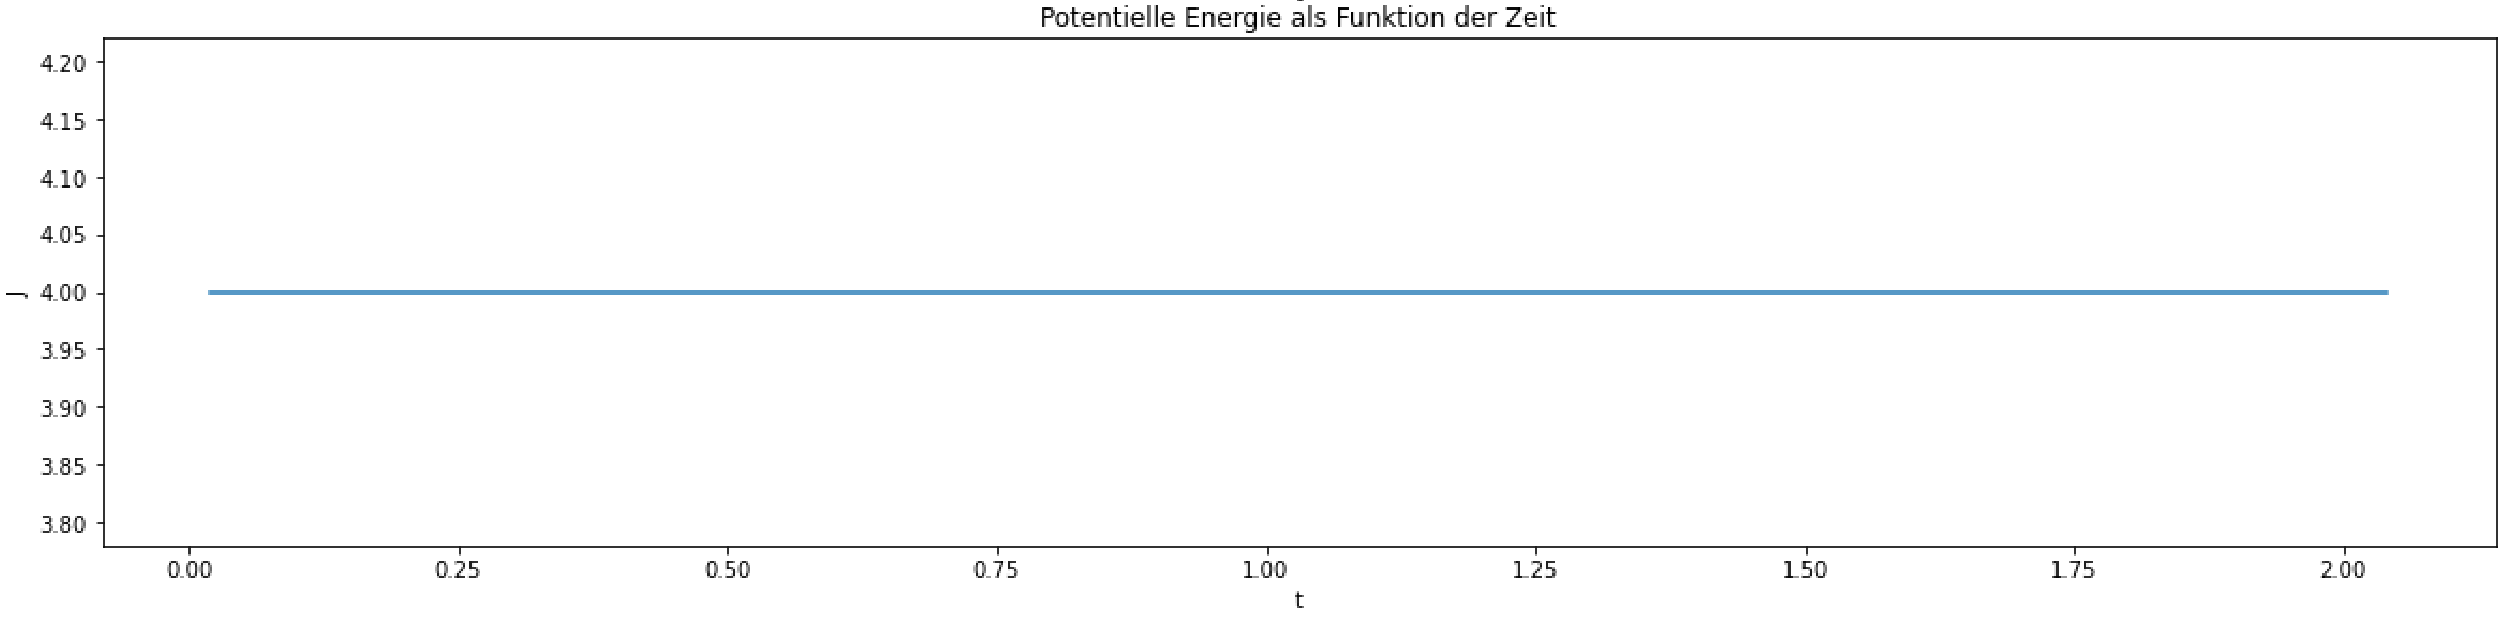
\includegraphics[width=155mm]{./images/Elastisch/PotentielleEnergieAlsFunktionDerZeit}}
            \caption{Potentielle Energie als Funktion der Zeit}
            \label{fig:PotentielleEnergieAlsFunktionDerZeit}
        \end{center}
    \end{figure}

    \subsection{Inelastisch}

    \begin{figure}[H]
        \begin{center}
            \centerline{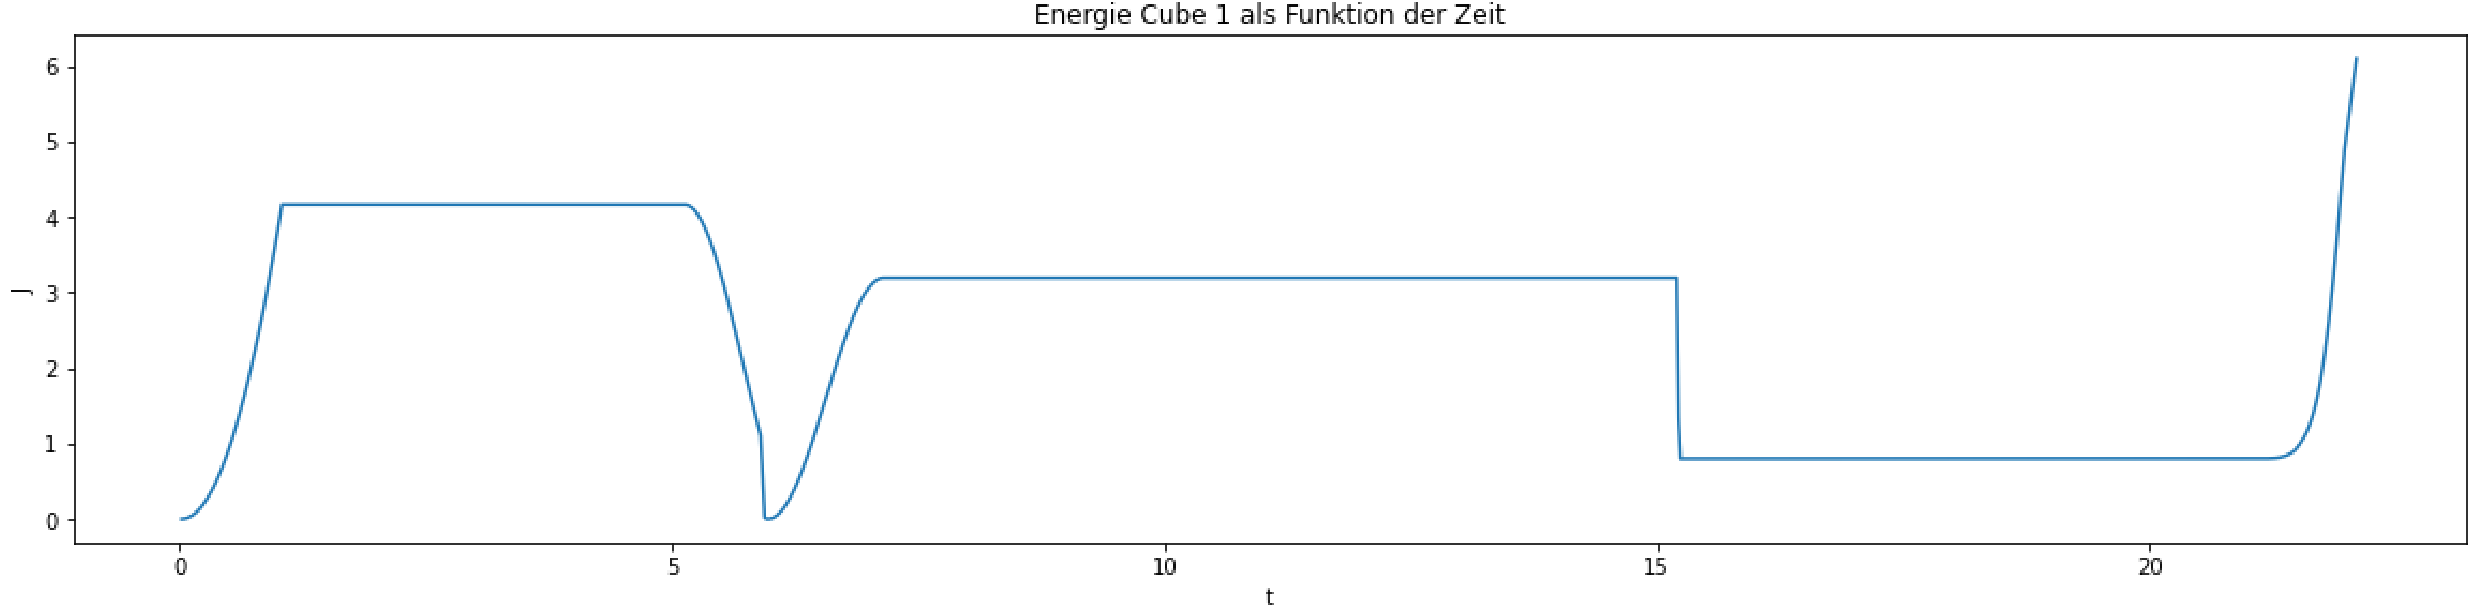
\includegraphics[width=155mm]{./images/Inelastisch/EnergieCube1AlsFunktionDerZeit}}
            \caption{Energie Cube 1 als Funktion der Zeit}
            \label{fig:EnergieCube1AlsFunktionDerZeit}
        \end{center}
    \end{figure}

    \begin{figure}[H]
        \begin{center}
            \centerline{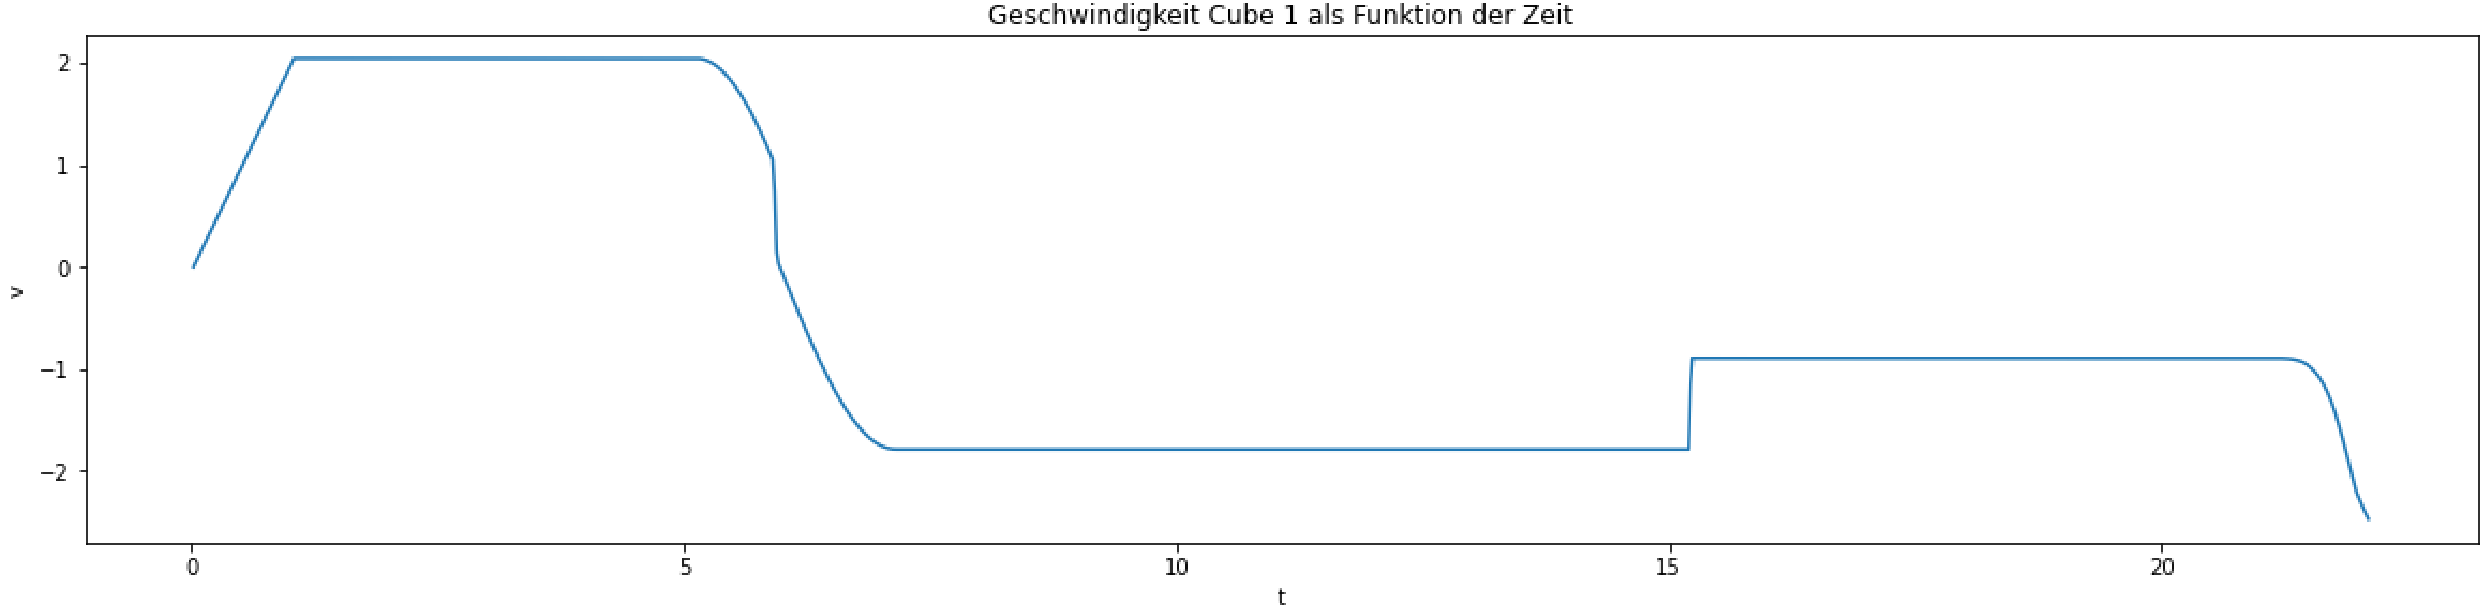
\includegraphics[width=155mm]{./images/Inelastisch/GeschwindigkeitCube1AlFunktionDerZeit}}
            \caption{Geschwindigkeit Cube 1 als Funktion der Zeit}
            \label{fig:GeschwindigkeitCube1AlFunktionDerZeit}
        \end{center}
    \end{figure}

    \begin{figure}[H]
        \begin{center}
            \centerline{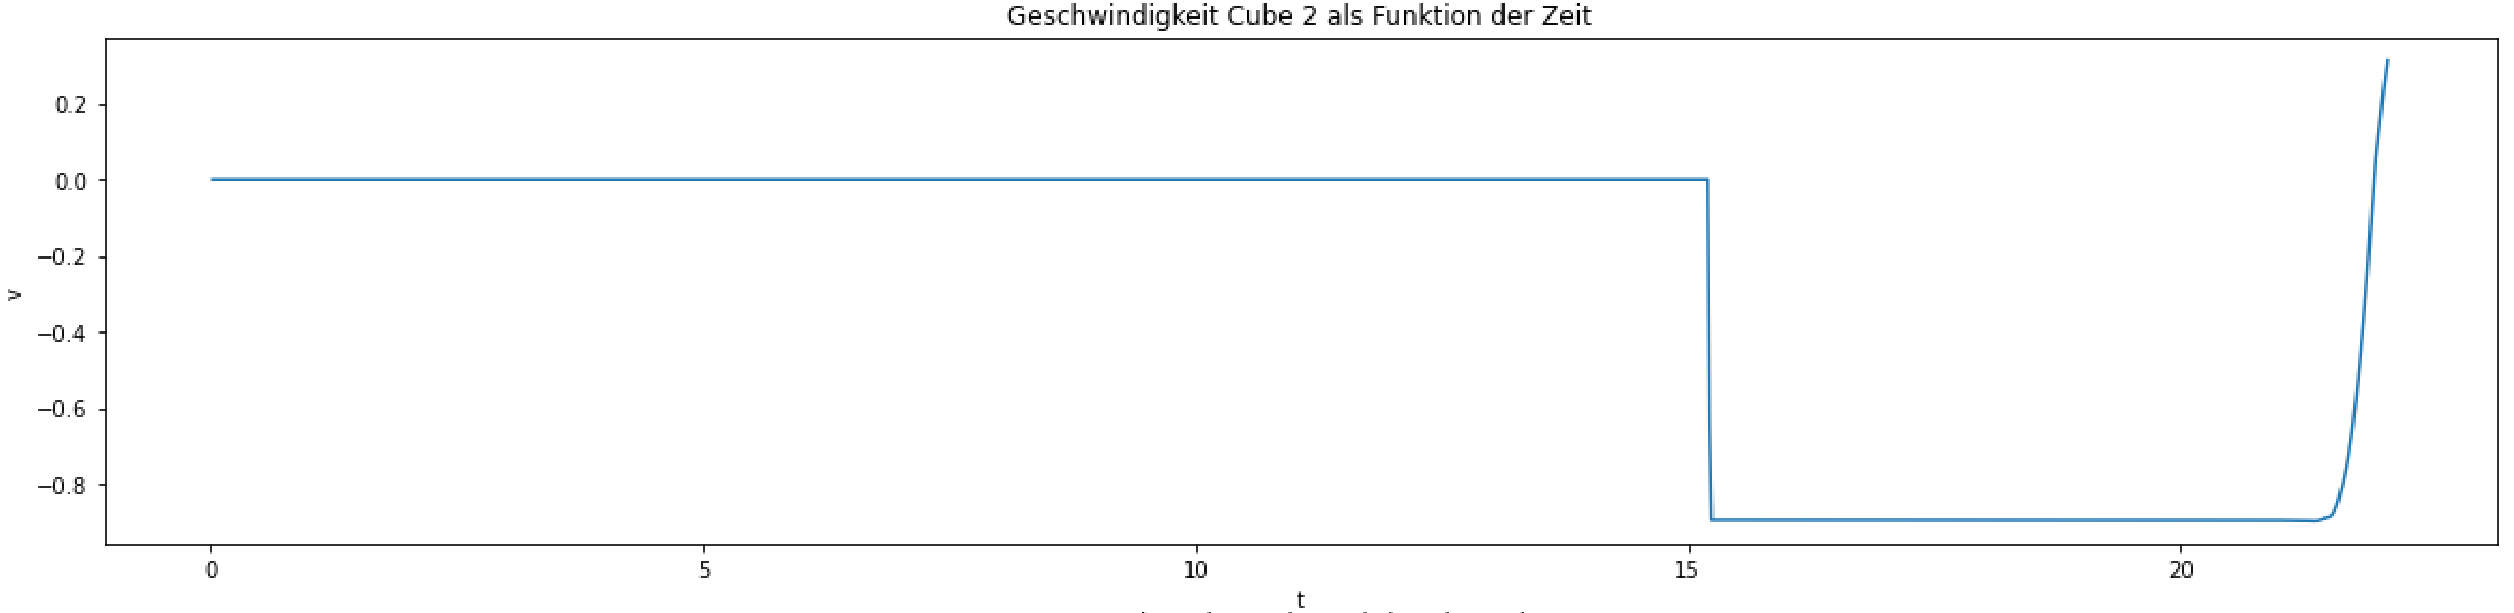
\includegraphics[width=155mm]{./images/Inelastisch/GeschwindigkeitCube2AlsFunktionDerZeit}}
            \caption{Geschwindigkeit Cube 2 als Funktion der Zeit}
            \label{fig:GeschwindigkeitCube2AlsFunktionDerZeit}
        \end{center}
    \end{figure}

    \begin{figure}[H]
        \begin{center}
            \centerline{\includegraphics[width=155mm]{./images/Inelastisch/OrtAlsFunktionDerZeit}}
            \caption{Ort als Funktion der Zeit}
            \label{fig:OrtAlsFunktionDerZeitInelastisch}
        \end{center}
    \end{figure}

    \subsection{Inelastisch}

\end{document}